%%%%%%%%%%%%%%%%%%%%%%%%%%%%%%%%%%%%%%%%%
% Short Sectioned Assignment
% LaTeX Template
% Version 1.0 (5/5/12)
%
% This template has been downloaded from:
% http://www.LaTeXTemplates.com
%
% Original author:
% Frits Wenneker (http://www.howtotex.com)
% License:
% CC BY-NC-SA 3.0 (http://creativecommons.org/licenses/by-nc-sa/3.0/)
%
%%%%%%%%%%%%%%%%%%%%%%%%%%%%%%%%%%%%%%%%%

%----------------------------------------------------------------------------------------
%	PACKAGES AND OTHER DOCUMENT CONFIGURATIONS
%----------------------------------------------------------------------------------------

\documentclass[paper=a4, fontsize=10pt, font=arial]{scrartcl} % A4 paper and 11pt font size

\usepackage[T1]{fontenc} % Use 8-bit encoding that has 256 glyphs
\usepackage{fourier} % Use the Adobe Utopia font for the document - comment this line to return to the LaTeX default
\usepackage[english]{babel} % English language/hyphenation
\usepackage{amsmath,amsfonts,amsthm} % Math packages
\usepackage{url}
\usepackage{sectsty} % Allows customizing section commands
\allsectionsfont{\centering \normalfont\scshape} % Make all sections centered, the default font and small caps
\usepackage{geometry}
\usepackage{float}
\usepackage{graphicx}
\usepackage{caption}
\usepackage{subcaption}
\usepackage{cite}
\usepackage{fancyhdr} % Custom headers and footers
%\bibliographystyle{unsrt}
\pagestyle{fancyplain} % Makes all pages in the document conform to the custom headers and footers
\fancyhead{} % No page header - if you want one, create it in the same way as the footers below
\footskip=0pt
\hoffset=0pt
\fancyfoot[L]{} % Empty left footer
\fancyfoot[C]{} % Empty center footer
\fancyfoot[R]{\thepage} % Page numbering for right footer
\renewcommand{\headrulewidth}{0pt} % Remove header underlines
\renewcommand{\footrulewidth}{0pt} % Remove footer underlines
\setlength{\headheight}{0pt} % Customize the height of the header
\setlength{\footheight}{0pt} % Customize the height of the header
\numberwithin{equation}{section} % Number equations within sections (i.e. 1.1, 1.2, 2.1, 2.2 instead of 1, 2, 3, 4)
\numberwithin{figure}{section} % Number figures within sections (i.e. 1.1, 1.2, 2.1, 2.2 instead of 1, 2, 3, 4)
\numberwithin{table}{section} % Number tables within sections (i.e. 1.1, 1.2, 2.1, 2.2 instead of 1, 2, 3, 4)
%\textheight=260cm
\setlength\parindent{11pt} % Removes all indentation from paragraphs - comment this line for an assignment with lots of text
\setlength{\parskip}{1em}
%----------------------------------------------------------------------------------------
%	TITLE SECTION
%----------------------------------------------------------------------------------------

\newcommand{\horrule}[1]{\rule{\linewidth}{#1}} % Create horizontal rule command with 1 argument of height

\title{	
\normalfont \normalsize 
\textsc{University of Derby, Department of Electronics, Mathematics \&\ Computing} \\ [25pt] % Your university, school and/or department name(s)
\horrule{0.5pt} \\[0.4cm] % Thin top horizontal rule
\huge The Impact of Reverberation Techniques on Immersion in Spatial Audio for Virtual Reality \\ % The assignment title
\horrule{2pt} \\[0.5cm] % Thick bottom horizontal rule
}

\author{Simon Durbridge} % Your name

\date{\normalsize\today} % Today's date or a custom date

\begin{document}

\maketitle % Print the title

%----------------------------------------------------------------------------------------
%	Abstract
%----------------------------------------------------------------------------------------

\section{Abstract}

\newpage

%----------------------------------------------------------------------------------------
%	Introduction
%----------------------------------------------------------------------------------------

\section{Introduction}

Increases in available computing power, and great strides in research and development have brought a new surge of interest to virtual reality (VR) applications. 
With the introduction of improved VR systems, such as Google Jump, Oculus, Vive and facebook360, using both high end computers, and mobile phone technology to provide immersive visualisation; Further steps are being taken to provide users with immersive sound environments~\cite{OculusCo41online}. 
These environments may be created in an  attempt to emulate real places, or to characterise fictional places.\par

A significant part of how humans identify with their surroundings, includes the perception of the reverberant characteristics of the surrounding area~\cite{rumsey2012spatial}. 
Cues such as the timing and strength of early reflections help humans to localize sound sources, as well as how far from the nearest boundaries the perceivers are. 
Some VR application development platforms provide a simplified model for how reverberation behaves in an audio system (negating early reflections), and may be an oversimplification when attempting to create an immersive audio experience that is tending towards the suspension of disbelief\footnote{This report is not intended to explore or discuss the artistic concept of the suspension of disbelief. For a discussion on this, please refer to CITE}.\par

The aim of this report is to introduce a testing method, to allow for the evaluation of different reverberation methods with respect to immersive VR audio. 
Initially, some theory behind reverberation and perception will be discussed. Following this, a brief description of current spatial audio techniques will be given. 
Finally, a testing framework will be proposed, in which subjects will evaluate different VR environments and reverb algorithms.


\newpage
%------------------------------------------------
\section{Reverberation \&\ Perception}
%---------------------------------------------
\subsection{Reverberation}

Reverberation (in a simplistic description), is the steady-state of diffusely scattered sound energy in a space due to the reflection of that energy from boundaries to a high order. Specifically, the amplitude of these reflections are such as to balance in amplitude with the steady state of the acoustic system, at or beyond the critical distance from a source (a classic analogy is given by Everest)~\cite{Everest2009}. 

\begin{figure}[H]
\centering
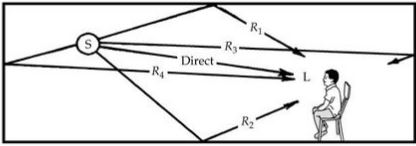
\includegraphics[width=0.4\textwidth]{reflection_diagran.jpg}
\centering
\caption{A conceptualisation of direct and reflected sound~\cite{Everest2009}}
\end{figure}

That is in contrast with strong reflections that may occur before excitation of the reverberant field (early reflections), or may occur later and above the steady state amplitude (echos)~\cite{Everest2009}. Early and strong reflections are of significant interest in this study, due to the cues humans recieve from perception of them. A reverberant sound field is often quantified by the decay time from steady state, to an amplitude of the steady state level $-60{dB}$. This is commonly described as the $RT_{60}$, and was proposed by WC Sabine in 1900. A more comprehensive description of reverberation and overview of the associated parameters is given by Rossing~\cite{rossing2007springer}. Further to this, the ratio of direct sound from a source to the amplitude of the reverberant field at any place in the sound field is also of interest~\cite{Begault1995}. A third parameter of interest is the clarity score, that is determined by the ratio between direct sound and an integration of the sound received directly from the source for some abritrary time (commonly 80ms). 

\begin{figure}[H]
\centering
\begin{subfigure}[b]{0.4\textwidth}
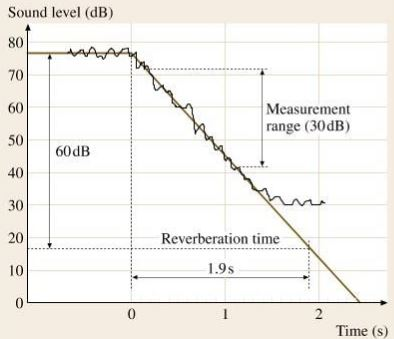
\includegraphics[width=\textwidth]{revertimedefinition.jpg}
\centering
\caption{An example graph of reverberation decay time $RT_{60}$}
\end{subfigure}
~
\begin{subfigure}[b]{0.4\textwidth}
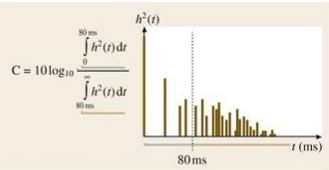
\includegraphics[width=\textwidth]{clarityscore.jpg}
\centering
\caption{An example of the calculation of Clatiry score}
\end{subfigure}
\caption{Graphics pertaining to quantification of reverberant sound ~\cite{rossing2007springer}}
\end{figure}

\subsection{Perception of Reflections}
There is a plethora of research and understanding of the objective quantification of reverberation~\cite{rossing2007springer}, less so about the subjective effects~\cite{Karjalainen2001} beyond the seminal studies of early reflections and level threshold shifts~\cite{Haas1972}. It may be argued that many facets of human auditory perception relate in some way to the perception of reverberation, the concepts of interest in this paper are those linked with localisation and perception of the auditory scene. Within these concepts are Haas/Precedence effect, and auditory masking.

The Haas effect is described as the first wave-front perceived by a listener, determines the source localisation in an auditory scene. The following reflections received within a 0.7 to 35mS window are integrated with the initial sound, such that the sound is given the impression of increased loudness, an increase in source width and tonal shifts of the percieved sound~\cite{Everest2009}. Beyond 40mS, following strong reflections are heard as echos. Begault~\cite{Begault1995} suggests that the precedence effect is the intrinsic mechanism  of the human auditory system, that allows for the localization of sound sources on a reverberant sound-field. Begault also suggests that there is a link between inter-aural time difference(ITD) perception for lateralization, and changes in apparent sound source 'width', suggesting a 5us to 1.5ms ITD 'window' within which a sound sources lateral location is determined. Another ascpet of note, is that if a sound source is occluded and the reflected sound is louder than the direct sound, the precedence effect is diminished~\cite{Wiggins2004}.

\begin{figure}[H]
\centering
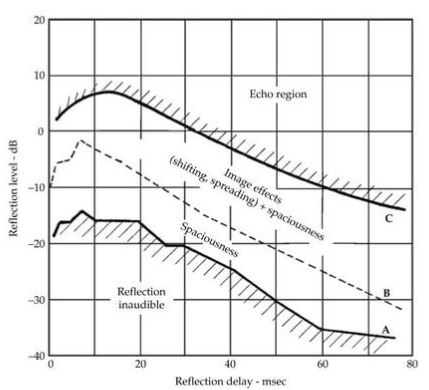
\includegraphics[width=0.4\textwidth]{precedence.jpg}
\caption{A plot of the window regions of precedence between reflection 'level' and delay~\cite{Everest2009}}
\end{figure}

Sigfried Linkwitz~\cite{Linkwitz2015} also discussed the idea that human perception of sound in enclosed spaces is powerful enough that given an appropriate sound source, a person can subconsciously differentiate between reflected sounds and the stereo sound-stage created by two sound sources.  The link is with auditory scene analysis. The argument is that more realistic reverberation modelling may provide a more realistic scene for our brains the analyse. 

Many of the texts referenced in this section of the report do not discuss auditory masking in great detail\footnote{Masking is noted by Begault, but not discussed}, though it may be of considerable importance when considering perception of noise-like sound. Auditory masking can be conceptualised as the time-envelope dependent blocking of new sounds being perceived, due to some other sound having already excited the inner ear. Specifically, sounds having already excited a portion of the bascilar membrane are thus stopping other sounds from being perceived as separate, that would otherwise excite the same portion of the bascilar membrane~\cite{Everest2009}. The bascilar membrane is often regarded as to be discretized into critical bands or equivalent rectangular bandwidths (ERB), and these bandwidths are different depending on sound level as well as centre frequency. General works by Moore ~\cite{Moore1996} should be reviewed for a more in-depth discussion of masking. The relevance of masking in this context, is that continuous noise is often used as a test signal in masking experiments, and steady-state reverberation may be similar to noise and thus cause masking of reflections and general reverberation. As such, creation of realistic reverberation may be important for masking in a natural way as opposed to having a spectrally dense or high amplitude artificial reverb that may cause excessive masking.

Echolocation\\

Timing \&\ Intensity\\

Concert Hall Reverberation\\

Aparant Source Width\\

Auditory Spaciousness\\

\subsection{Reverberation Algorithms}

Derived Reverberation\\

Geometric Modelling\\

Wave Modelling\\

%------------------------------------------------
\section{Ambisonic Spatial Audio for Virtual Reality}
\subsubsection{Audio Spatial Perception}

Spatial Cues\\
ITD\\

ILD\\

HRTFS\\

Direct to Reverberant Ratio\\

Precedence\\

Auditory Scene Analysis

\subsubsection{Ambisonics}
%\paragraph{Heading on level 4 (paragraph)}

the concept of ambisonics\\


\section{Experiment Protocol}



Users will be asked to evaluate 5 different instances of VR environments, and determine which audio is from the real environment.

Karjalainen \textit{et al}~\cite{Karjalainen2001} undertook a study into the perception of late reverberation, using a perceptual model to reinforce listening test data.

%----------------------------------------------------------------------------------------
%	PROBLEM 2
%----------------------------------------------------------------------------------------

\section{Lists}

%------------------------------------------------

\subsection{Example of list (3*itemize)}
\begin{itemize}
	\item First item in a list 
		\begin{itemize}
		\item First item in a list 
			\begin{itemize}
			\item First item in a list 
			\item Second item in a list 
			\end{itemize}
		\item Second item in a list 
		\end{itemize}
	\item Second item in a list 
\end{itemize}

%------------------------------------------------

\subsection{Example of list (enumerate)}
\begin{enumerate}
\item First item in a list 
\item Second item in a list 
\item Third item in a list
\end{enumerate}

\begin{align} 
\begin{split}
(x+y)^3 	&= (x+y)^2(x+y)\\
&=(x^2+2xy+y^2)(x+y)\\
&=(x^3+2x^2y+xy^2) + (x^2y+2xy^2+y^3)\\
&=x^3+3x^2y+3xy^2+y^3
\end{split}					
\end{align}

\begin{align}
A = 
\begin{bmatrix}
A_{11} & A_{21} \\
A_{21} & A_{22}
\end{bmatrix}
\end{align}

\begin{center}
$RT_{60} = \frac{0.161 A}{Sa}$\\
\end{center}


%----------------------------------------------------------------------------------------
\newpage
\section{References}

\bibliography{mylibrary}{}
\bibliographystyle{plain}

\end{document}